\section{Introduction}
\label{sect:introduction}

Supersymmetry \cite{Martin:1997ns} (SUSY) is one of the most promising extensions of the 
standard model of the elementary particles (SM) which solves both the 
quadratic divergencies and hierarchy problems simultaneously. It introduces a new symmetry between the bosons and fermions and 
for every particle a sparticle is defined which is exactly the same, but differ in spin by 1/2. 
%Since the super particles are not discovered yet, the supersymmetry should be a broken symmetry. 
%Various mechanisms are introduced to break the symmetry softly without changing the other interesting features of the theory.
Extensive searches at the CERN LHC have pushed the mass of the colored SUSY particles much beyond the previous expectations \cite{susyPhyRes}. 
Looking for the electroweak production of sparticles is therefore well motivated to not miss possible SUSY signals in a corner. 


A search for new physics using the full 2012 data is documented in this note. 
Although the search is sensitive to any high scale 
new physics with a missing transverse energy (\MET), an R-parity conserving SUSY model is used 
to illustrate the performance of the method.

The electroweak production of the SUSY particles with the leptonic final state was studies previously \cite{CMS-PAS-SUS-13-006}.
In the current analysis, due to the special role of the third generation of the sparticles, events with two tau leptons in the final state 
accompanying with \MET are considered.
The two tau leptons can be generated in the cascade of the staus or charginos:
\begin{linenomath}
\begin{equation}
p + p \rightarrow \PSGcpDo +\PSGcmDo ~~\mathrm{or}~~  p + p \rightarrow \sTau + \sTau,
\end{equation}
\end{linenomath}
when 
\begin{linenomath}
\begin{equation}
\PSGcpDo \rightarrow \sTau + \nu ~~\mathrm{or}~~  \PSGcpDo \rightarrow \sNu_{\tau} + \tau,
\end{equation}
\end{linenomath}
and 
\begin{linenomath}
\begin{equation}
\sTau \rightarrow \tau + \PSGczDo ~~\mathrm{or}~~  \sNu_{\tau} \rightarrow \nu + \PSGczDo.
\end{equation}
\end{linenomath}
The $\PSGczDo$ can not be detected and appears as \MET.
Figure \ref{fig:Productions} shows the main processes that can generate our favorite final state.
\begin{figure}[!Hhtb]
\centering
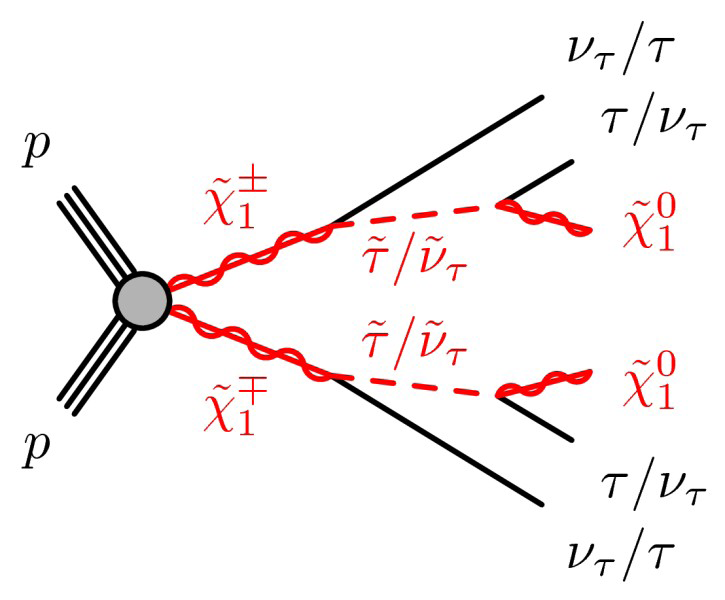
\includegraphics[width=0.49\textwidth]{Introductionfigs/DiChargino.png}
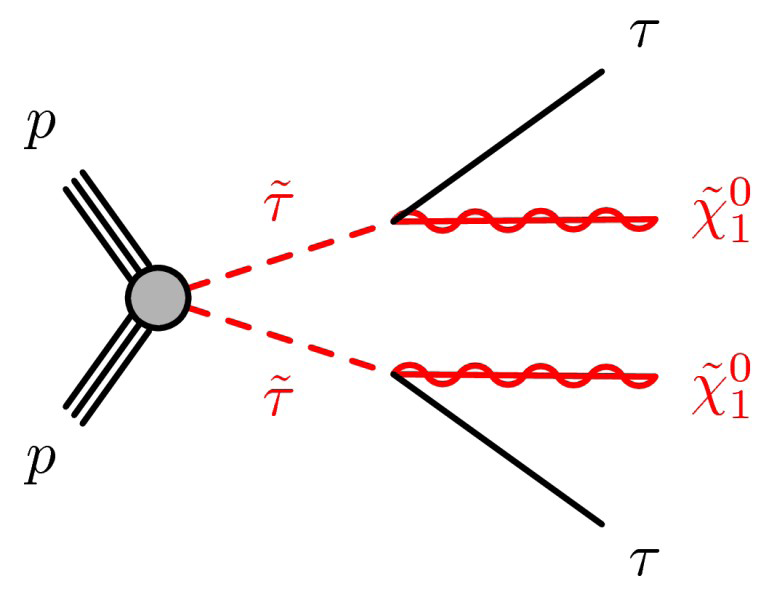
\includegraphics[width=0.49\textwidth]{Introductionfigs/DiSTau.png}
\caption{Schematic production of double tau from chargino pair and stau pair.}
\label{fig:Productions}
\end{figure}
The production cross section of $\PSGcpDo\PSGcmDo$ is more than one order of magnitude higher than the
production cross section of \sTau\sTau in the same mass of \sTau and \PSGcpDo,  
for example for a 150 \GeVcc \sTau or \PSGcpDo, the cross section 
of the pair production of the particles is 27 $fb$ and 1170 $fb$, respectively. Due to the higher cross section through this note, 
we mainly focus on the $\PSGcpDo\PSGcmDo$ production. 

%In the context of MSSM, supersymmetric objects are produced in pairs to conserve R-parity quantum number. Therefore in the production of charginos from proton-proton collisions, one may consider the following interaction $$pp\rightarrow\PSGcpDo\PSGcmDo\rightarrow\sTau^{+}\nu_\tau \sTau^{-}\nu_\tau\rightarrow\tau^{+}\PSGczDo\nu_\tau\tau^{-}\PSGczDo\nu_\tau\rightarrow\tau^{+}\tau^{-} + 2\,\PSGczDo + 2\,\nu_\tau.$$ In the detector, what can be observed are only 2 tau leptons plus missing transverse energy from the presence of neturinos and neutralinos in the final state.\\ 
The tau leptons decay leptonically ($e$ or $\mu$), in 35\% of the time, or decay via hadrons, which occurs in 65\% of the cases. Since there are two tau leptons in the final state, the probability of having $\PSGcpDo\PSGcmDo \rightarrow \hadtau+e/\mu+\MET$ is about 46\%, while the probability for $\PSGcpDo\PSGcmDo \rightarrow \hadtau+\hadtau+\MET$ to occur is about 42\%. Hereafter, final states containing a lepton are referred to as $\leptonTau$ channel and those events where the two taus decay via hadrons are referred to as $\tauTau$. The selection cuts to enhance $\tauTau$ events will be discussed in Section~\ref{sect:tauTauCuts}. The list of cuts to select $\leptonTau$ events can be found in Section~\ref{sect:leptonTauCuts}.\\     

The search variable is the stransverse mass (\mttwo) which is the natural extension of the known transverse mass (\mt) to a case 
when two massive particles with equal mass are created in pairs and decay via a chain of jets and leptons to two 
invisible particles, similar to our case.
%In the case of R-parity conserving SUSY, the Lightest Supersymmetric Particle (LSP), \PSGczDo in our scenario, 
%escapes  detection and appears as \MET.

The distribution of \mttwo reflects the scale of the produced particles and is much higher for sparticles
compared to the SM particles. Hence, SUSY should appear as an excess in the tail of the \mttwo distribution.
It was shown previously \cite{MT2_2011} and \cite{CMS-PAS-SUS-13-006} that \mttwo is a powerful variable to search for SUSY in both
hadronic and leptonic final states.

The current note is organized as follows, after introduction in the next section the \mttwo variable is introduced. Different datasets 
and objects used in this analysis are discussed in sections \ref{sect:dataMC} and \ref{sect:objdef}. The events selections for different channels
are shown in section \ref{sect:cuts}. A detailed study of the SM backgrounds is presented in section \ref{sect:bkg}. Section \ref{sect:sys} 
is devoted to evaluation of the systematic uncertainties. The final numbers and their statistical interpretation is presented in 
section \ref{sect:stat} and finally section \ref{sect:conclusion} concludes the note.





